\section{Labeling Tool}\label{sec:labeling-tool}

Um die Erstellung und Verwaltung von gelabelten \ac{BPMN}-Prozessmodellen zu erleichtern, wurde eine Webapplikation entwickelt. Mit dieser können \ac{BPMN}-Testfälle erstellt, bearbeitet und Aktivitäten mit Labeln versehen werden. Wichtige Funktionen des Labeling-Tools umfassen:

\begin{itemize}
    \item Anlegen und Verwalten von Datensätzen.
    \item Erstellung beliebig vieler Testfälle pro Datensatz.
    \item Direkte Bearbeitung von \ac{BPMN}-Modellen im Browser mittels BPMN.io \cite{bpmnio}.
    \item Labeling-Modus, in dem Aktivitäten als \ac{DSGVO}-kritisch markiert werden können. Optional kann eine Begründung für die Markierung angegeben werden.
    \item Persistente Speicherung der annotierten Testfälle in einer Datenbank für die spätere Nutzung im Evaluationsframework (siehe Kapitel \ref{ch:evaluationsframework}).
\end{itemize}

Abbildung \ref{fig:labeling-editor} zeigt den Labeling-Editor: Hier können Anwender Prozessmodelle erstellen und Aktivitäten im Labeling-Modus direkt als kritisch markieren. Optional kann für jede markierte Aktivität eine Begründung eingegeben werden. Diese Begründung ist ausschließlich als Hilfe für den Anwender gedacht, um die eigene Entscheidung zu dokumentieren. Die Begründung wird nicht in der Evaluierung berücksichtigt.

\begin{figure}
    \centering
    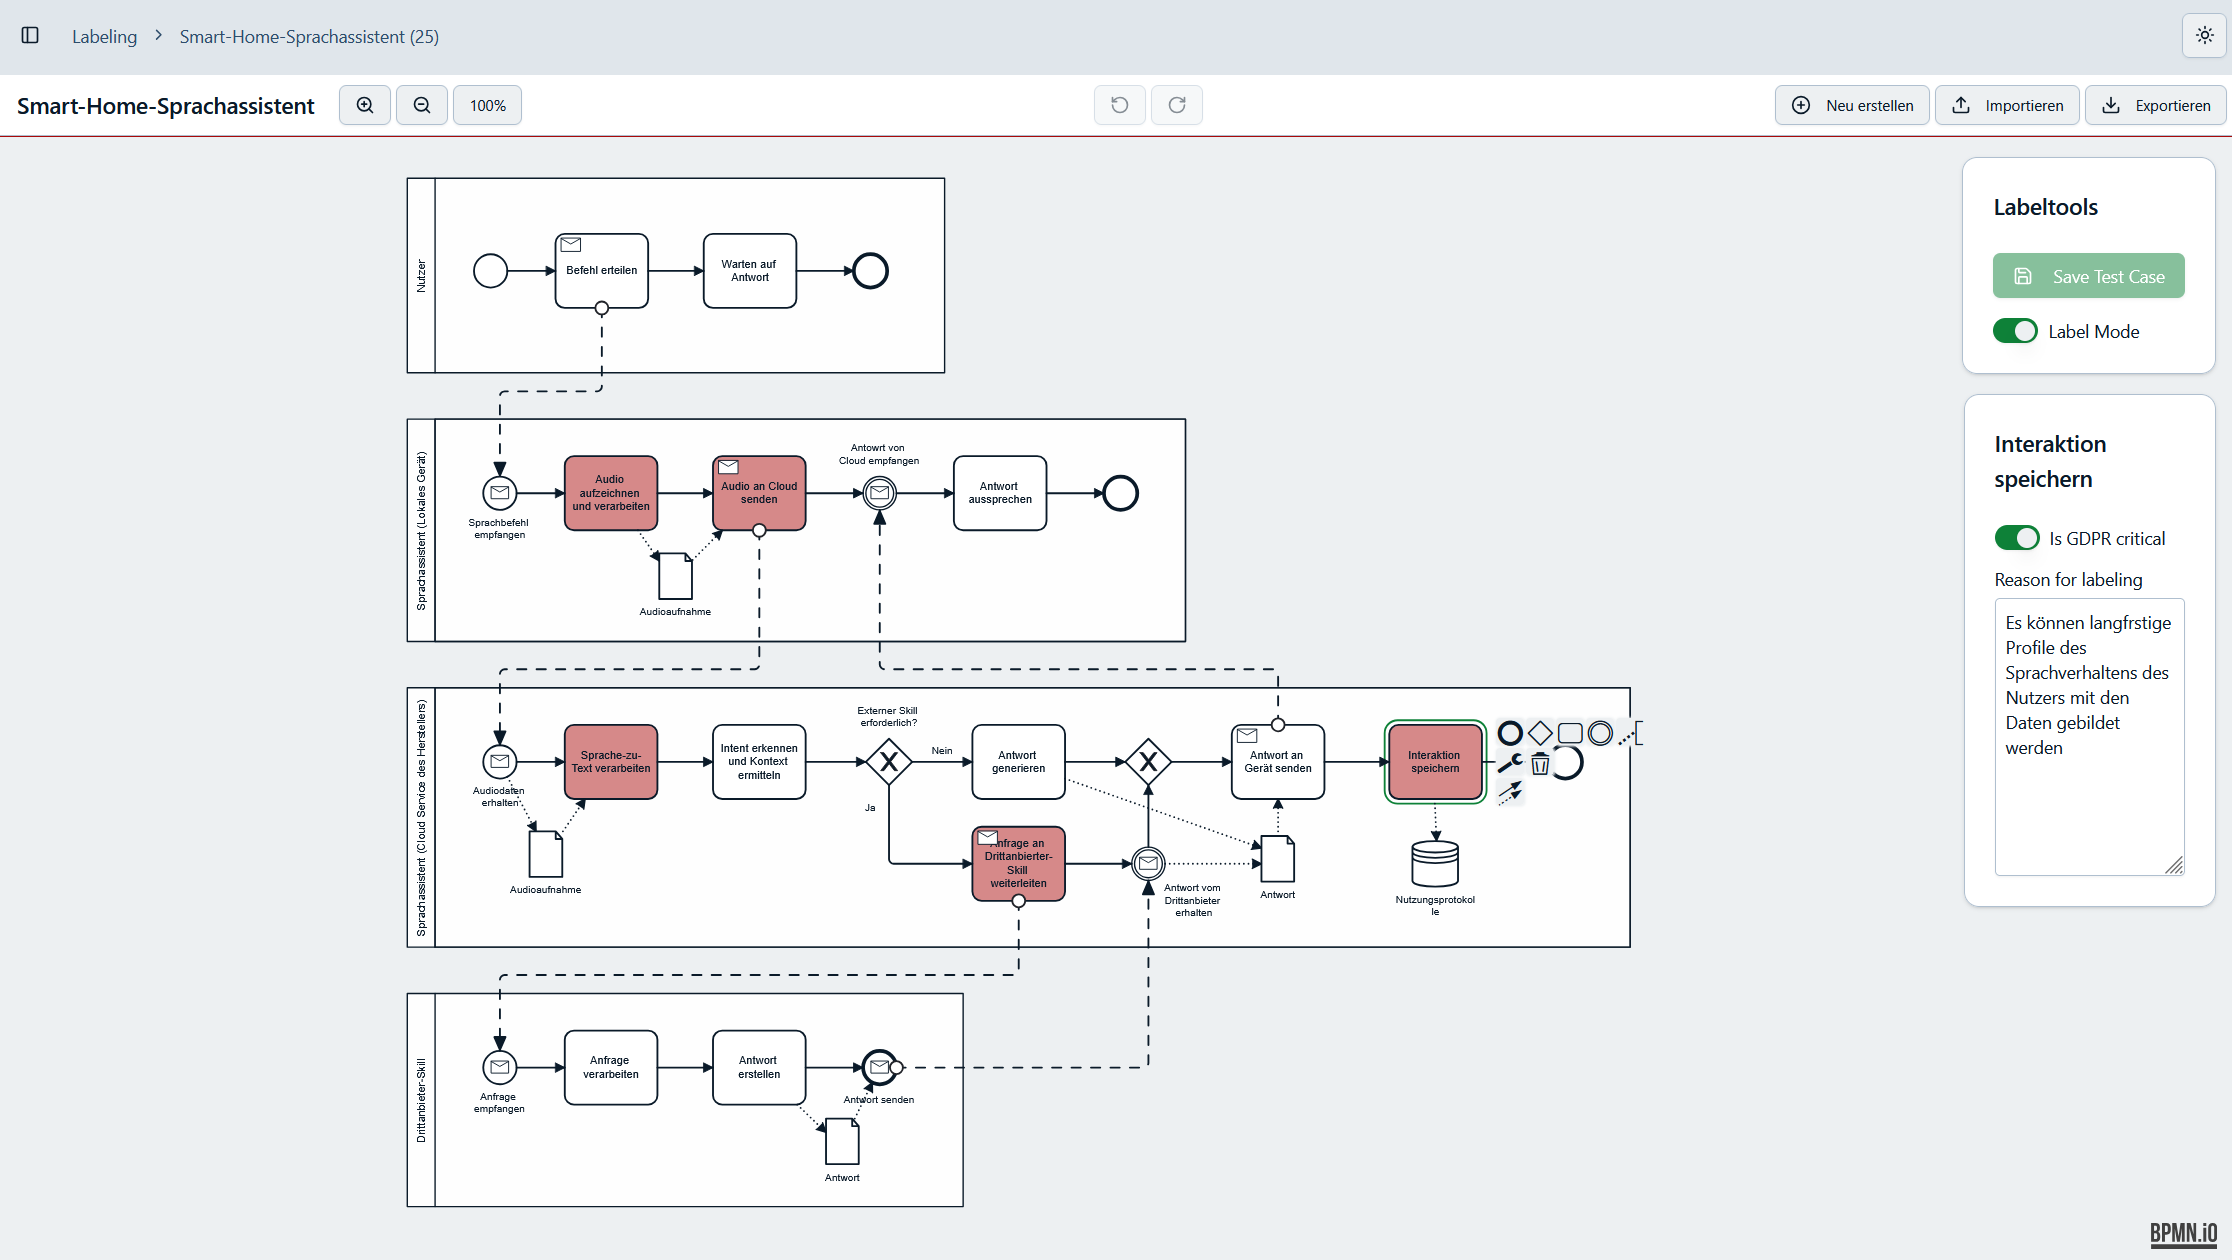
\includegraphics[width=\textwidth]{images/labeling/labeling-editor}
    \caption{Labeling-Editor im Labeling-Modus mit exemplarischem Modell.}
    \label{fig:labeling-editor}
\end{figure}

In der Übersicht der Datensätze aus Abbildung \ref{fig:labeling-datasets} sind alle angelegten Datensätze und zugehörigen Testfälle aufgelistet. Von hier aus können neue Datensätze und Testfälle erstellt sowie bestehende bearbeitet werden.

\begin{figure}
    \centering
    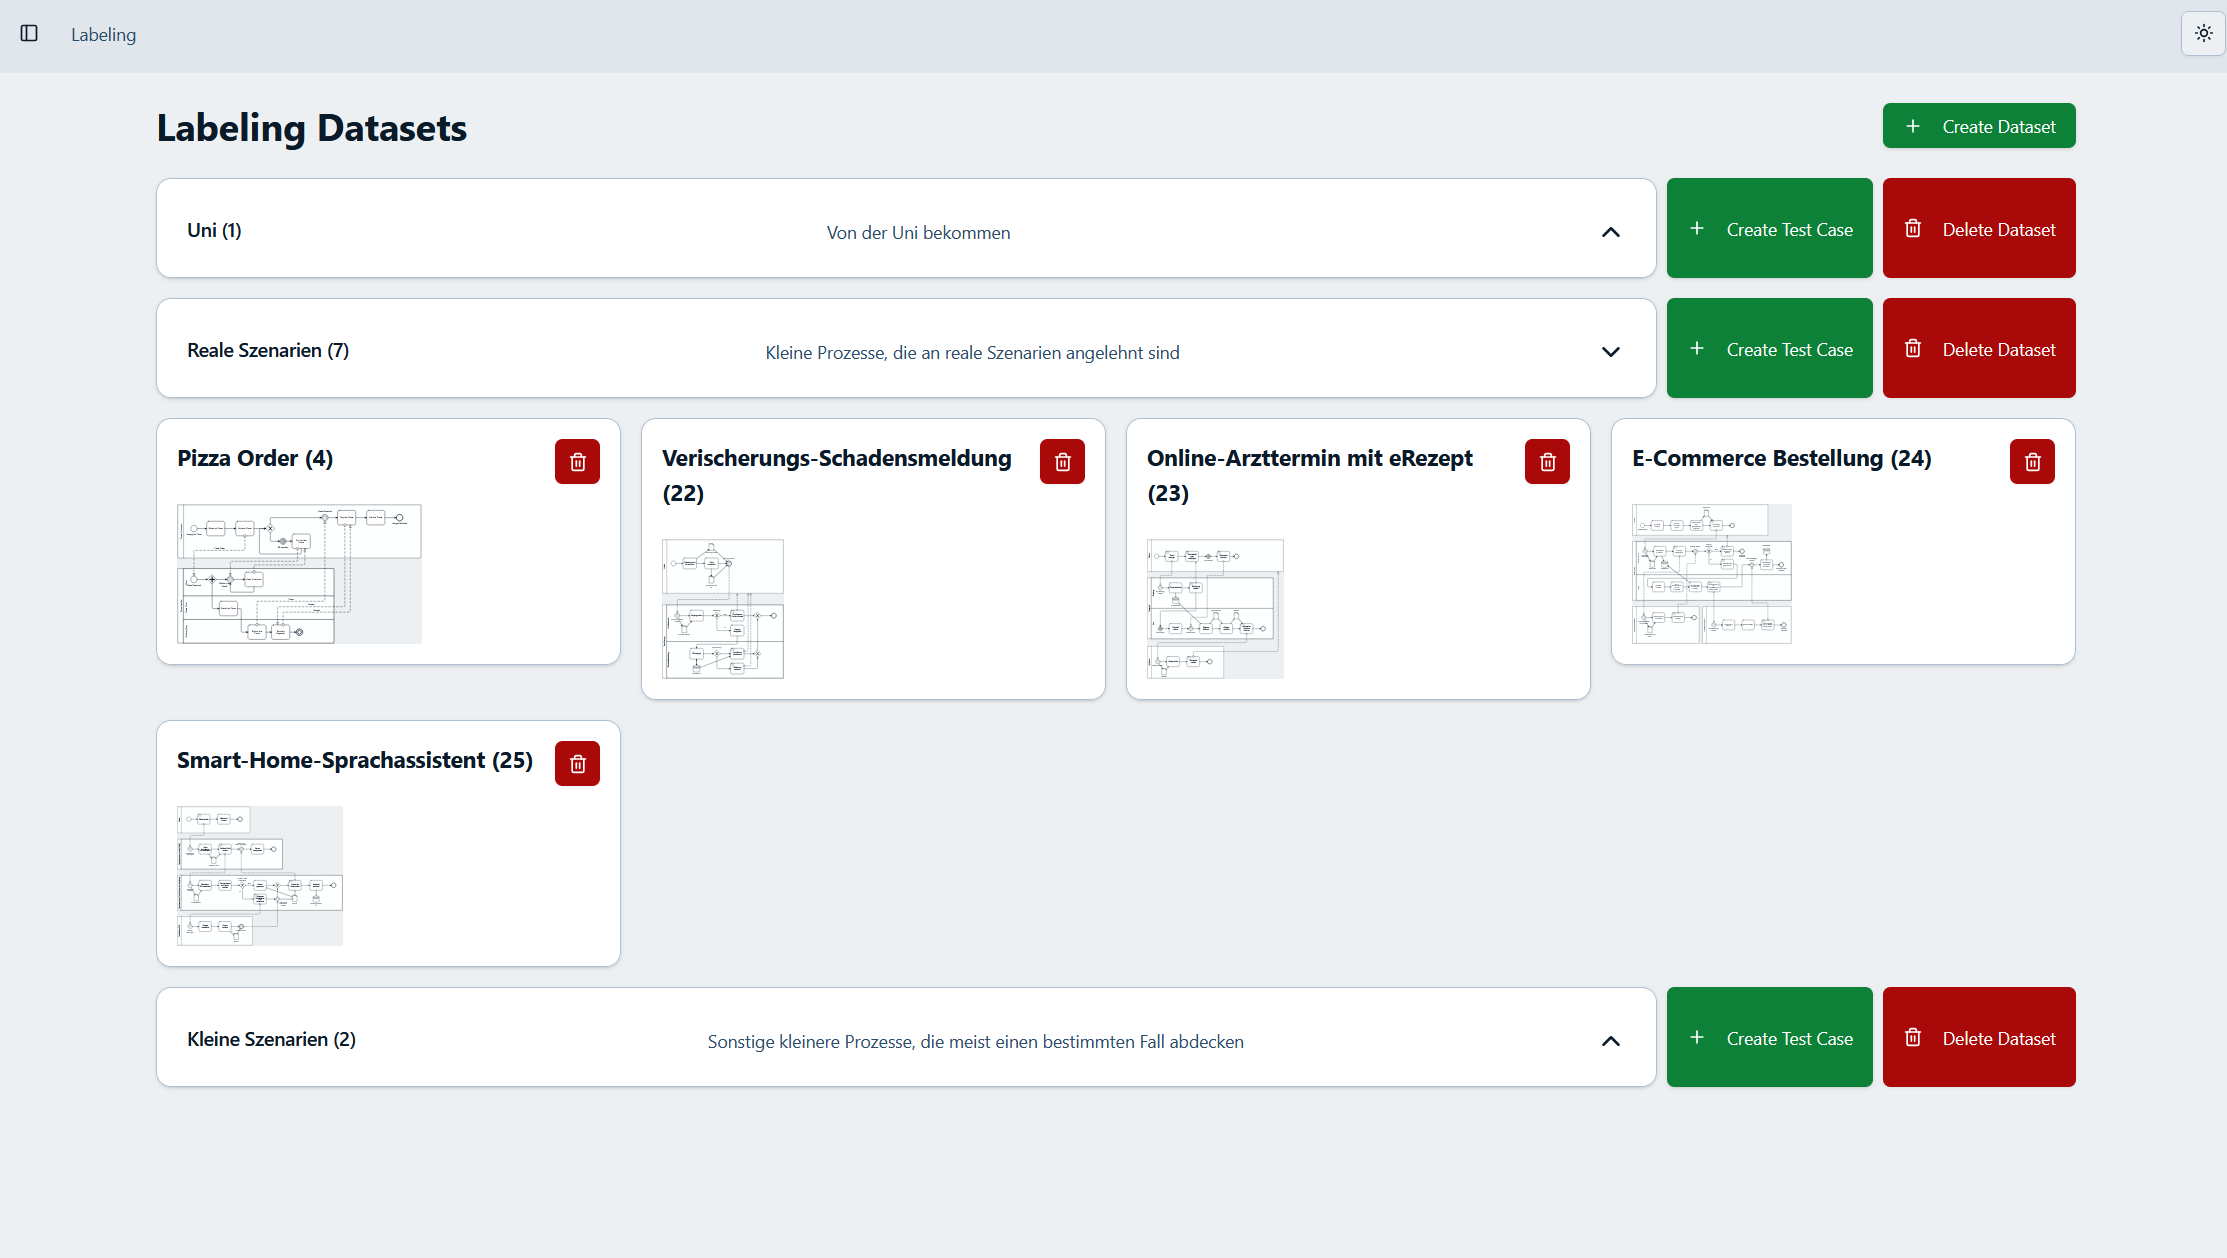
\includegraphics[width=\textwidth]{images/labeling/labeling-datasets}
    \caption{Übersicht der Datensätze im Labeling-Tool.}
    \label{fig:labeling-datasets}
\end{figure}